\documentclass[12pt, titlepage]{article}

\usepackage{fullpage}
\usepackage[round]{natbib}
\usepackage{multirow}
\usepackage{booktabs}
\usepackage{tabularx}
\usepackage{graphicx}
\usepackage{float}
\usepackage{hyperref}
\hypersetup{
    colorlinks,
    citecolor=blue,
    filecolor=black,
    linkcolor=red,
    urlcolor=blue
}

%% Comments

\usepackage{color}

\newif\ifcomments\commentstrue %displays comments
%\newif\ifcomments\commentsfalse %so that comments do not display

\ifcomments
\newcommand{\authornote}[3]{\textcolor{#1}{[#3 ---#2]}}
\newcommand{\todo}[1]{\textcolor{red}{[TODO: #1]}}
\else
\newcommand{\authornote}[3]{}
\newcommand{\todo}[1]{}
\fi

\newcommand{\wss}[1]{\authornote{blue}{SS}{#1}} 
\newcommand{\plt}[1]{\authornote{magenta}{TPLT}{#1}} %For explanation of the template
\newcommand{\an}[1]{\authornote{cyan}{Author}{#1}}

%% Common Parts

\newcommand{\progname}{ProgName} % PUT YOUR PROGRAM NAME HERE
\newcommand{\authname}{Team \#, Team Name
\\ Student 1 name
\\ Student 2 name
\\ Student 3 name
\\ Student 4 name} % AUTHOR NAMES                  

\usepackage{hyperref}
    \hypersetup{colorlinks=true, linkcolor=blue, citecolor=blue, filecolor=blue,
                urlcolor=blue, unicode=false}
    \urlstyle{same}
                                


\newcounter{acnum}
\newcommand{\actheacnum}{AC\theacnum}
\newcommand{\acref}[1]{AC\ref{#1}}

\newcounter{ucnum}
\newcommand{\uctheucnum}{UC\theucnum}
\newcommand{\uref}[1]{UC\ref{#1}}

\newcounter{mnum}
\newcommand{\mthemnum}{M\themnum}
\newcommand{\mref}[1]{M\ref{#1}}

\begin{document}

\title{Module Guide for \progname{}} 
\author{\authname}
\date{\today}

\maketitle

\pagenumbering{roman}

\section{Revision History}

\begin{tabularx}{\textwidth}{p{3cm}p{2cm}X}
\toprule {\bf Date} & {\bf Version} & {\bf Notes}\\
\midrule
Date 1 & 1.0 & Notes\\
Date 2 & 1.1 & Notes\\
\bottomrule
\end{tabularx}

\newpage

\section{Reference Material}

This section records information for easy reference.

\subsection{Abbreviations and Acronyms}

\renewcommand{\arraystretch}{1.2}
\begin{tabular}{l l} 
  \toprule		
  \textbf{symbol} & \textbf{description}\\
  \midrule 
  AC & Anticipated Change\\
  DAG & Directed Acyclic Graph \\
  M & Module \\
  MG & Module Guide \\
  OS & Operating System \\
  R & Requirement\\
  SC & Scientific Computing \\
  SRS & Software Requirements Specification\\
  \progname & Explanation of program name\\
  UC & Unlikely Change \\
  \wss{etc.} & \wss{...}\\
  \bottomrule
\end{tabular}\\

\newpage

\tableofcontents

\listoftables

\listoffigures

\newpage

\pagenumbering{arabic}

\section{Introduction}

Decomposing a system into modules is a commonly accepted approach to developing
software.  A module is a work assignment for a programmer or programming
team~\citep{ParnasEtAl1984}.  We advocate a decomposition
based on the principle of information hiding~\citep{Parnas1972a}.  This
principle supports design for change, because the ``secrets'' that each module
hides represent likely future changes.  Design for change is valuable in SC,
where modifications are frequent, especially during initial development as the
solution space is explored.  

Our design follows the rules layed out by \citet{ParnasEtAl1984}, as follows:
\begin{itemize}
\item System details that are likely to change independently should be the
  secrets of separate modules.
\item Each data structure is implemented in only one module.
\item Any other program that requires information stored in a module's data
  structures must obtain it by calling access programs belonging to that module.
\end{itemize}

After completing the first stage of the design, the Software Requirements
Specification (SRS), the Module Guide (MG) is developed~\citep{ParnasEtAl1984}. The MG
specifies the modular structure of the system and is intended to allow both
designers and maintainers to easily identify the parts of the software.  The
potential readers of this document are as follows:

\begin{itemize}
\item New project members: This document can be a guide for a new project member
  to easily understand the overall structure and quickly find the
  relevant modules they are searching for.
\item Maintainers: The hierarchical structure of the module guide improves the
  maintainers' understanding when they need to make changes to the system. It is
  important for a maintainer to update the relevant sections of the document
  after changes have been made.
\item Designers: Once the module guide has been written, it can be used to
  check for consistency, feasibility, and flexibility. Designers can verify the
  system in various ways, such as consistency among modules, feasibility of the
  decomposition, and flexibility of the design.
\end{itemize}

The rest of the document is organized as follows. Section
\ref{SecChange} lists the anticipated and unlikely changes of the software
requirements. Section \ref{SecMH} summarizes the module decomposition that
was constructed according to the likely changes. Section \ref{SecConnection}
specifies the connections between the software requirements and the
modules. Section \ref{SecMD} gives a detailed description of the
modules. Section \ref{SecTM} includes two traceability matrices. One checks
the completeness of the design against the requirements provided in the SRS. The
other shows the relation between anticipated changes and the modules. Section
\ref{SecUse} describes the use relation between modules.

\section{Anticipated and Unlikely Changes} \label{SecChange}

This section lists possible changes to the system. The changes are categorized as either anticipated or unlikely, based on their probability and potential impact. Anticipated changes represent areas of the system expected to evolve due to regular updates or new requirements. Unlikely changes are those that would require significant rework and are less probable given the current context.

\subsection{Anticipated Changes} \label{SecAchange}

Anticipated changes are the source of information hidden within the modules. These changes are expected to occur as part of system updates or user feedback and are designed to be handled with minimal impact on the overall structure.

\begin{description}
\item[\refstepcounter{acnum} \actheacnum \label{acHardware}:] The specific hardware on which the software is hosted. 
\begin{itemize}
    \item Examples include MES-provided laptops with Windows 10 and above-average specifications or the potential transition to cloud-hosted environments like Azure or AWS. 
    \item Impact: Hardware dependencies are encapsulated in the hardware-hiding module to isolate changes and avoid propagation to higher-level modules.
\end{itemize}

\item[\refstepcounter{acnum} \actheacnum \label{acInput}:] The format of input data, such as receipts or invoices uploaded by student groups. 
\begin{itemize}
    \item Examples: Adding support for new file formats (e.g., PDFs, images, CSVs) or incorporating OCR (Optical Character Recognition) for scanned documents.
    \item Impact: Changes to input formats affect only the Input Format and Data Validation Modules, which transform raw input into system-compatible data structures.
\end{itemize}

\item[\refstepcounter{acnum} \actheacnum \label{acNotifications}:] Notification methods, such as expanding delivery channels. 
\begin{itemize}
    \item Examples: Adding SMS notifications, push alerts via a mobile app, or integration with messaging platforms like Slack or Teams.
    \item Impact: The Notifications System Module handles all updates to notification methods, ensuring other modules remain unaffected.
\end{itemize}

\item[\refstepcounter{acnum} \actheacnum \label{acWorkflow}:] Changes to the workflow for reimbursement request approvals. 
\begin{itemize}
    \item Examples: Modifying multi-level approval processes, incorporating dynamic routing based on the requester’s department, or enabling automated rejections for incomplete submissions.
    \item Impact: The Approval Workflow Module encapsulates these decisions, minimizing disruptions to related modules.
\end{itemize}

\item[\refstepcounter{acnum} \actheacnum \label{acAudit}:] Requirements for audit log duration and format. 
\begin{itemize}
    \item Examples: Updating log retention policies from 6 months to 2 years or adding additional metadata to logs for enhanced traceability.
    \item Impact: Changes are confined to the Audit and Compliance Module, ensuring audit functionality evolves independently.
\end{itemize}
\end{description}

\subsection{Unlikely Changes} \label{SecUchange}

Unlikely changes are less probable due to their disruptive nature or because they contradict established constraints and design principles. While the system design is modular, accommodating these changes would require significant rework across multiple modules.

\begin{description}
\item[\refstepcounter{ucnum} \uctheucnum \label{ucDevice}:] Supported devices. 
\begin{itemize}
    \item Examples: Expanding compatibility to entirely new platforms like gaming consoles or wearables.
    \item Impact: Extensive updates to the Graphical User Interface (GUI) and hardware-hiding modules would be required.
\end{itemize}

\item[\refstepcounter{ucnum} \uctheucnum \label{ucTechStack}:] The technology stack used. 
\begin{itemize}
    \item Examples: Replacing TypeScript and Next.js with entirely different frameworks or programming languages.
    \item Impact: This change would affect almost all modules, requiring a complete system overhaul and significant developer retraining.
\end{itemize}

\item[\refstepcounter{ucnum} \uctheucnum \label{ucPolicy}:] Legal or compliance policies. 
\begin{itemize}
    \item Examples: Abandoning compliance with AODA (Accessibility for Ontarians with Disabilities Act) or PIPEDA (Personal Information Protection and Electronic Documents Act).
    \item Impact: Changes would cascade through the Policy and Compliance Management Module, potentially invalidating existing processes and documentation.
\end{itemize}
\end{description}

\section{Module Hierarchy} \label{SecMH}

This section provides an overview of the module design. Modules are organized in a hierarchy to encapsulate secrets and ensure clear boundaries of responsibilities, following the principles of information hiding. Each module is classified into one of three categories: Hardware-Hiding, Behaviour-Hiding, and Software Decision. The hierarchy reflects how modules interact and rely on one another, ensuring scalability, maintainability, and ease of future modifications. A detailed breakdown is provided in Table \ref{TblMH}.

\begin{description}
\item [\refstepcounter{mnum} \mthemnum \label{mHH}:] 
\textbf{Hardware-Hiding Module} \\
\textbf{Secrets:} Abstracts the interaction with the underlying hardware components, including database connections and file I/O.\\
\textbf{Responsibilities:} Provides foundational services such as data storage and retrieval, ensuring consistent access and isolation from hardware-specific details.\\
\textbf{Implemented By:} Relational database systems (e.g., PostgreSQL) and middleware APIs.

\item [\refstepcounter{mnum} \mthemnum \label{mBH}:] 
\textbf{Behaviour-Hiding Module} \\
\textbf{Secrets:} Implements the core functional behaviors of the system, encapsulating workflows and interactions as defined by the SRS.\\
\textbf{Responsibilities:} Manages user interactions, financial workflows, compliance auditing, and communication systems. Each submodule addresses specific business logic and user requirements.\\
\textbf{Implemented By:} TypeScript-based backend services integrated with the frontend application.

\item [\refstepcounter{mnum} \mthemnum \label{mSD}:] 
\textbf{Software Decision Module} \\
\textbf{Secrets:} Encapsulates design decisions that are based on algorithms, heuristics, or data structures, which are independent of user interactions.\\
\textbf{Responsibilities:} Supports development and operational processes, including testing, validation, and CI/CD pipelines. Ensures system robustness through automated validation and testing mechanisms.\\
\textbf{Implemented By:} GitHub Actions for CI/CD, Jest for test automation, and custom validation libraries.
\end{description}

\begin{table}[H] 
\centering
\renewcommand{\arraystretch}{1.5}
\begin{tabular}{p{0.3\textwidth} p{0.6\textwidth}}
\toprule
\textbf{Level 1} & \textbf{Level 2}\\
\midrule

{Hardware-Hiding Module} & Database Interaction Layer \\ 
\midrule

\multirow{7}{0.3\textwidth}{Behaviour-Hiding Module} & Reimbursement Submission\\
& Reimbursement Review and Approval\\
& Audit and Compliance Module\\
& Budget Dashboard\\
& Notification System\\
& User Management\\ 
& Financial Reporting\\
\midrule

\multirow{3}{0.3\textwidth}{Software Decision Module} & CI/CD Integration\\
& Test Automation Framework\\
& Data Validation Module\\
\bottomrule
\end{tabular}
\caption{Module Hierarchy}
\label{TblMH}
\end{table}


\section{Connection Between Requirements and Design}

The design of the MES-ERP system has been structured to ensure that the requirements outlined in the Software Requirements Specification (SRS) are met comprehensively. Table~\ref{tab:req-to-modules} illustrates the connection between the requirements and the modules designed to fulfill them.

\begin{table}[h!]
\centering
\caption{Connection Between Requirements and Modules}
\label{tab:req-to-modules}
\begin{tabular}{|p{4cm}|p{8cm}|}
\hline
\textbf{Requirement (R)} & \textbf{Modules} \\
\hline
R1: Secure Authentication & User Authentication \& Profile Management Module \\
\hline
R2: Expense Submission \& Tracking & Expense Submission \& Tracking Module \\
\hline
R3: Budget Validation & Budget and Funding Management Module \\
\hline
R4: Approval Workflow & Approval Workflow and Review Module \\
\hline
R5: Notifications & Notifications \& Communication Module \\
\hline
R6: Compliance & Policy \& Compliance Management Module \\
\hline
R7: Reporting & Reporting and Analytics Module \\
\hline
R8: Administrative Tools & Administrator and Configuration Panel Module \\
\hline
\end{tabular}
\end{table}

\subsection{Design Decisions for Each Requirement}

\begin{itemize}
    \item \textbf{R1: Secure Authentication}
    \begin{itemize}
        \item \textbf{Module}: User Authentication \& Profile Management Module
        \item \textbf{Design Decision}: Implements secure login with session timeouts, role-based access control, and account lockout mechanisms.
    \end{itemize}
    
    \item \textbf{R2: Expense Submission \& Tracking}
    \begin{itemize}
        \item \textbf{Module}: Expense Submission \& Tracking Module
        \item \textbf{Design Decision}: Provides forms for submission, receipt uploads, and tracking expense status.
    \end{itemize}
    
    \item \textbf{R3: Budget Validation}
    \begin{itemize}
        \item \textbf{Module}: Budget and Funding Management Module
        \item \textbf{Design Decision}: Ensures expense requests do not exceed departmental budgets and integrates with the financial system.
    \end{itemize}
    
    \item \textbf{R4: Approval Workflow}
    \begin{itemize}
        \item \textbf{Module}: Approval Workflow and Review Module
        \item \textbf{Design Decision}: Implements dynamic routing for approvals and notifications for pending actions.
    \end{itemize}
    
    \item \textbf{R5: Notifications}
    \begin{itemize}
        \item \textbf{Module}: Notifications \& Communication Module
        \item \textbf{Design Decision}: Sends alerts via email, SMS, and dashboard notifications for system events.
    \end{itemize}
    
    \item \textbf{R6: Compliance}
    \begin{itemize}
        \item \textbf{Module}: Policy \& Compliance Management Module
        \item \textbf{Design Decision}: Validates expense requests against predefined policies to ensure compliance with regulations.
    \end{itemize}
    
    \item \textbf{R7: Reporting}
    \begin{itemize}
        \item \textbf{Module}: Reporting and Analytics Module
        \item \textbf{Design Decision}: Generates detailed reports in PDF/CSV format for expense tracking and system usage.
    \end{itemize}
    
    \item \textbf{R8: Administrative Tools}
    \begin{itemize}
        \item \textbf{Module}: Administrator and Configuration Panel Module
        \item \textbf{Design Decision}: Enables administrators to manage user roles, configure approval workflows, and access system logs.
    \end{itemize}
\end{itemize}

\section{Module Decomposition}

The MES-ERP system is designed following the principle of \textit{information hiding}, which ensures that each module encapsulates decisions likely to change independently. The modules are organized into a hierarchy, with higher-level modules relying on lower-level ones for functionality. This hierarchy forms a directed acyclic graph (DAG). Figure~\ref{fig:module-decomposition} illustrates the module decomposition.

\subsection{Module Levels}

\begin{itemize}
    \item \textbf{Hardware-Hiding Modules}
    \begin{itemize}
        \item \textbf{Database Module}: Provides a foundational interface for storing and retrieving data. It serves as the core data storage system, used by nearly all other modules.
    \end{itemize}
    
    \item \textbf{Behavior-Hiding Modules}
    \begin{itemize}
        \item \textbf{User Authentication \& Profile Management Module}: Manages secure login, user sessions, and profiles.
        \item \textbf{Expense Submission \& Tracking Module}: Handles expense submission, receipt uploads, and tracking.
        \item \textbf{Policy \& Compliance Management Module}: Ensures submitted expenses comply with organizational policies.
    \end{itemize}
    
    \item \textbf{Software Decision Modules}
    \begin{itemize}
        \item \textbf{Approval Workflow and Review Module}: Manages dynamic workflows for expense approvals.
        \item \textbf{Budget and Funding Management Module}: Validates budgets and tracks funding.
        \item \textbf{Reporting and Analytics Module}: Provides reporting tools and analytics for system data.
    \end{itemize}
    
    \item \textbf{Presentation Layer Modules}
    \begin{itemize}
        \item \textbf{Graphical User Interface (GUI) Module}: Interacts with users by displaying data and capturing inputs.
        \item \textbf{Notifications \& Communication Module}: Sends alerts and notifications to users via email, SMS, or the dashboard.
    \end{itemize}
\end{itemize}

\subsection{Use Relations Between Modules}

\begin{itemize}
    \item \textbf{Database Module}
    \begin{itemize}
        \item \textbf{Used By}: 
        User Authentication \& Profile Management, Expense Submission \& Tracking, Budget and Funding Management, Approval Workflow and Review, Notifications \& Communication, Reporting and Analytics, Policy \& Compliance Management.
        \item \textbf{Purpose}: Acts as the central data storage and retrieval system.
    \end{itemize}
    
    \item \textbf{User Authentication \& Profile Management Module}
    \begin{itemize}
        \item \textbf{Used By}: Approval Workflow and Review, Notifications \& Communication, GUI Module.
        \item \textbf{Purpose}: Provides secure access to the system and maintains user roles and profiles.
    \end{itemize}
    
    \item \textbf{Expense Submission \& Tracking Module}
    \begin{itemize}
        \item \textbf{Used By}: Approval Workflow and Review, Budget and Funding Management, Notifications \& Communication, Reporting and Analytics.
        \item \textbf{Purpose}: Handles expense submissions, categorization, and tracking.
    \end{itemize}
    
    \item \textbf{Budget and Funding Management Module}
    \begin{itemize}
        \item \textbf{Used By}: Expense Submission \& Tracking, Approval Workflow and Review, Notifications \& Communication.
        \item \textbf{Purpose}: Validates and updates budgets associated with submitted expenses.
    \end{itemize}
    
    \item \textbf{Approval Workflow and Review Module}
    \begin{itemize}
        \item \textbf{Used By}: Notifications \& Communication, GUI Module.
        \item \textbf{Purpose}: Implements dynamic routing and rules for approving expenses.
    \end{itemize}
    
    \item \textbf{Notifications \& Communication Module}
    \begin{itemize}
        \item \textbf{Used By}: GUI Module, all other modules requiring alerts or updates.
        \item \textbf{Purpose}: Sends notifications and alerts via email, SMS, or dashboard.
    \end{itemize}
    
    \item \textbf{Reporting and Analytics Module}
    \begin{itemize}
        \item \textbf{Used By}: GUI Module, Administrator and Configuration Panel.
        \item \textbf{Purpose}: Provides analytics and reporting tools for system data.
    \end{itemize}
    
    \item \textbf{Graphical User Interface (GUI) Module}
    \begin{itemize}
        \item \textbf{Used By}: End users interacting with the system.
        \item \textbf{Relies On}: Backend modules to fetch and display data.
        \item \textbf{Purpose}: Displays system data and handles user interactions.
    \end{itemize}
\end{itemize}

\subsection{Hardware Hiding Modules (\mref{mHH})}

\begin{description}
\item[Secrets:]The data structure and algorithm used to implement the virtual
  hardware.
\item[Services:]Serves as a virtual hardware used by the rest of the
  system. This module provides the interface between the hardware and the
  software. So, the system can use it to display outputs or to accept inputs.
\item[Implemented By:] OS
\end{description}

\subsection{Behaviour-Hiding Module}

\begin{description}
\item[Secrets:]The contents of the required behaviours.
\item[Services:]Includes programs that provide externally visible behaviour of
  the system as specified in the software requirements specification (SRS)
  documents. This module serves as a communication layer between the
  hardware-hiding module and the software decision module. The programs in this
  module will need to change if there are changes in the SRS.
\item[Implemented By:] --
\end{description}

\subsubsection{Input Format Module (\mref{mInput})}

\begin{description}
\item[Secrets:]The format and structure of the input data.
\item[Services:]Converts the input data into the data structure used by the
  input parameters module.
\item[Implemented By:] [Your Program Name Here]
\item[Type of Module:] [Record, Library, Abstract Object, or Abstract Data Type]
  [Information to include for leaf modules in the decomposition by secrets tree.]
\end{description}

\subsubsection{Etc.}


\subsection{Software Decision Module}

\begin{description}
\item[Secrets:] The design decision based on mathematical theorems, physical
  facts, or programming considerations. The secrets of this module are
  \emph{not} described in the SRS.
\item[Services:] Includes data structure and algorithms used in the system that
  do not provide direct interaction with the user. 
  % Changes in these modules are more likely to be motivated by a desire to
  % improve performance than by externally imposed changes.
\item[Implemented By:] --
\end{description}

\subsubsection{Etc.}

\section{Traceability Matrix}

This section outlines the anticipated changes to the MES-ERP system and identifies the modules that would be impacted by each change. The traceability matrix maps these anticipated changes to the affected modules, ensuring alignment with the principle of \textit{information hiding}.

\subsection{Anticipated Changes to Modules}

Table~\ref{tab:anticipated-changes} provides a traceability matrix that lists the anticipated changes and their associated modules.

\begin{table}[h!]
\centering
\caption{Traceability Matrix: Anticipated Changes to Modules}
\label{tab:anticipated-changes}
\begin{tabular}{|p{6cm}|p{8cm}|}
\hline
\textbf{Anticipated Change (AC)} & \textbf{Affected Modules} \\
\hline
AC1: Changes in Authentication Protocols & User Authentication \& Profile Management Module \\
\hline
AC2: New Expense Categories & Expense Submission \& Tracking Module \\
\hline
AC3: Budget Limits Adjustment & Budget and Funding Management Module \\
\hline
AC4: Workflow Modifications & Approval Workflow and Review Module \\
\hline
AC5: New Notification Methods & Notifications \& Communication Module \\
\hline
AC6: Policy Updates & Policy \& Compliance Management Module \\
\hline
AC7: Report Formats or Types & Reporting and Analytics Module \\
\hline
AC8: Additional Admin Features & Administrator and Configuration Panel Module \\
\hline
\end{tabular}
\end{table}

\subsection{Impact of Anticipated Changes}

\begin{itemize}
    \item \textbf{AC1: Changes in Authentication Protocols}
    \begin{itemize}
        \item \textbf{Affected Module}: User Authentication \& Profile Management Module
        \item \textbf{Impact}: Updates to the \texttt{authenticate()} function to support new protocols (e.g., multi-factor authentication) and modifications to constants like session timeouts.
        \item \textbf{Mitigation}: Encapsulation of authentication logic minimizes impact on other modules.
    \end{itemize}
    
    \item \textbf{AC2: New Expense Categories}
    \begin{itemize}
        \item \textbf{Affected Module}: Expense Submission \& Tracking Module
        \item \textbf{Impact}: Updates to the \texttt{EXPENSE\_CATEGORIES} constant and adjustments to the \texttt{categorizeExpense()} function.
        \item \textbf{Mitigation}: Modular handling of categories allows isolated changes without affecting other modules.
    \end{itemize}
    
    \item \textbf{AC3: Budget Limits Adjustment}
    \begin{itemize}
        \item \textbf{Affected Module}: Budget and Funding Management Module
        \item \textbf{Impact}: Modifications to the \texttt{MAX\_BUDGET} constant and related validation logic.
        \item \textbf{Mitigation}: Centralized budget handling simplifies updates.
    \end{itemize}
    
    \item \textbf{AC4: Workflow Modifications}
    \begin{itemize}
        \item \textbf{Affected Module}: Approval Workflow and Review Module
        \item \textbf{Impact}: Updates to \texttt{routeRequest()} and \texttt{updateStatus()} functions for new workflow rules.
        \item \textbf{Mitigation}: Dynamic routing logic supports flexible workflow updates.
    \end{itemize}
    
    \item \textbf{AC5: New Notification Methods}
    \begin{itemize}
        \item \textbf{Affected Module}: Notifications \& Communication Module
        \item \textbf{Impact}: Addition of new constants (e.g., \texttt{NOTIFICATION\_TYPES}) and updates to notification functions.
        \item \textbf{Mitigation}: Modular notification handling allows easy integration of new methods.
    \end{itemize}
    
    \item \textbf{AC6: Policy Updates}
    \begin{itemize}
        \item \textbf{Affected Module}: Policy \& Compliance Management Module
        \item \textbf{Impact}: Updates to \texttt{validateRequest()} to handle new policy rules and thresholds.
        \item \textbf{Mitigation}: Encapsulation of policy logic ensures minimal impact on unrelated modules.
    \end{itemize}
    
    \item \textbf{AC7: Report Formats or Types}
    \begin{itemize}
        \item \textbf{Affected Module}: Reporting and Analytics Module
        \item \textbf{Impact}: Modifications to \texttt{generateReport()} to support new formats or metrics.
        \item \textbf{Mitigation}: Flexible report generation logic minimizes system-wide impact.
    \end{itemize}
    
    \item \textbf{AC8: Additional Admin Features}
    \begin{itemize}
        \item \textbf{Affected Module}: Administrator and Configuration Panel Module
        \item \textbf{Impact}: New access programs (e.g., \texttt{addFeature()}, \texttt{updateRolePermissions()}).
        \item \textbf{Mitigation}: Well-defined admin tools enable straightforward updates.
    \end{itemize}
\end{itemize}


\section{Use Hierarchy Between Modules} \label{SecUse}

In this section, the uses hierarchy between modules is
provided. \citet{Parnas1978} said of two programs A and B that A {\em uses} B if
correct execution of B may be necessary for A to complete the task described in
its specification. That is, A {\em uses} B if there exist situations in which
the correct functioning of A depends upon the availability of a correct
implementation of B.  Figure \ref{FigUH} illustrates the use relation between
the modules. It can be seen that the graph is a directed acyclic graph
(DAG). Each level of the hierarchy offers a testable and usable subset of the
system, and modules in the higher level of the hierarchy are essentially simpler
because they use modules from the lower levels.

\begin{figure}[H]
  \centering
  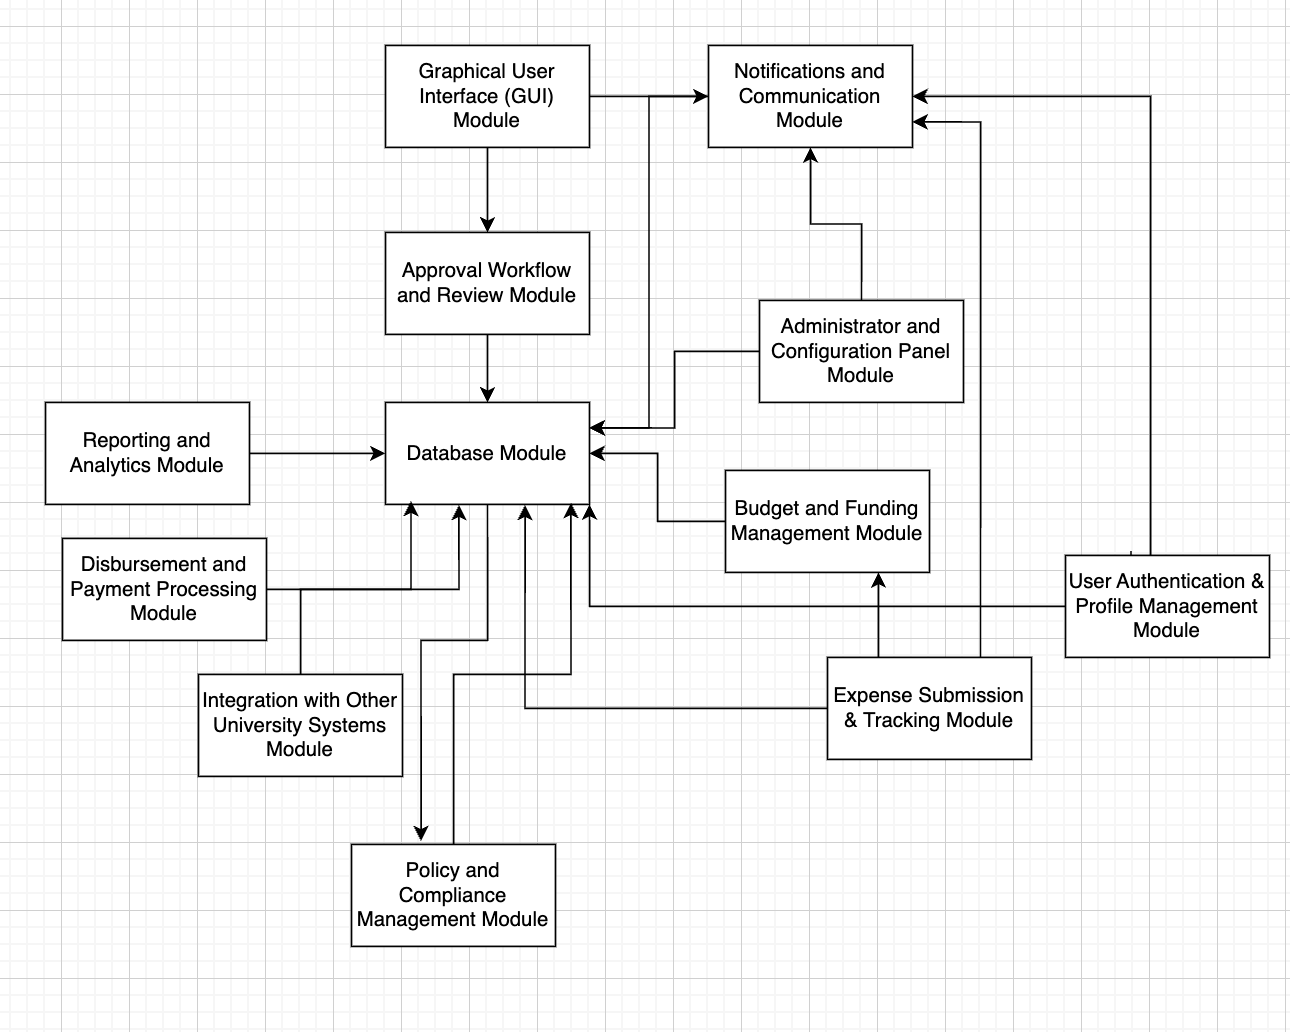
\includegraphics[width=1\textwidth]{img/diagram.png}
  \caption{Module Hierarchy}
  \label{fig:diagram}
\end{figure}


%\section*{References}

\section{User Interfaces} 

\subsection{Dashboard}
\begin{figure}[H]
    \centering
    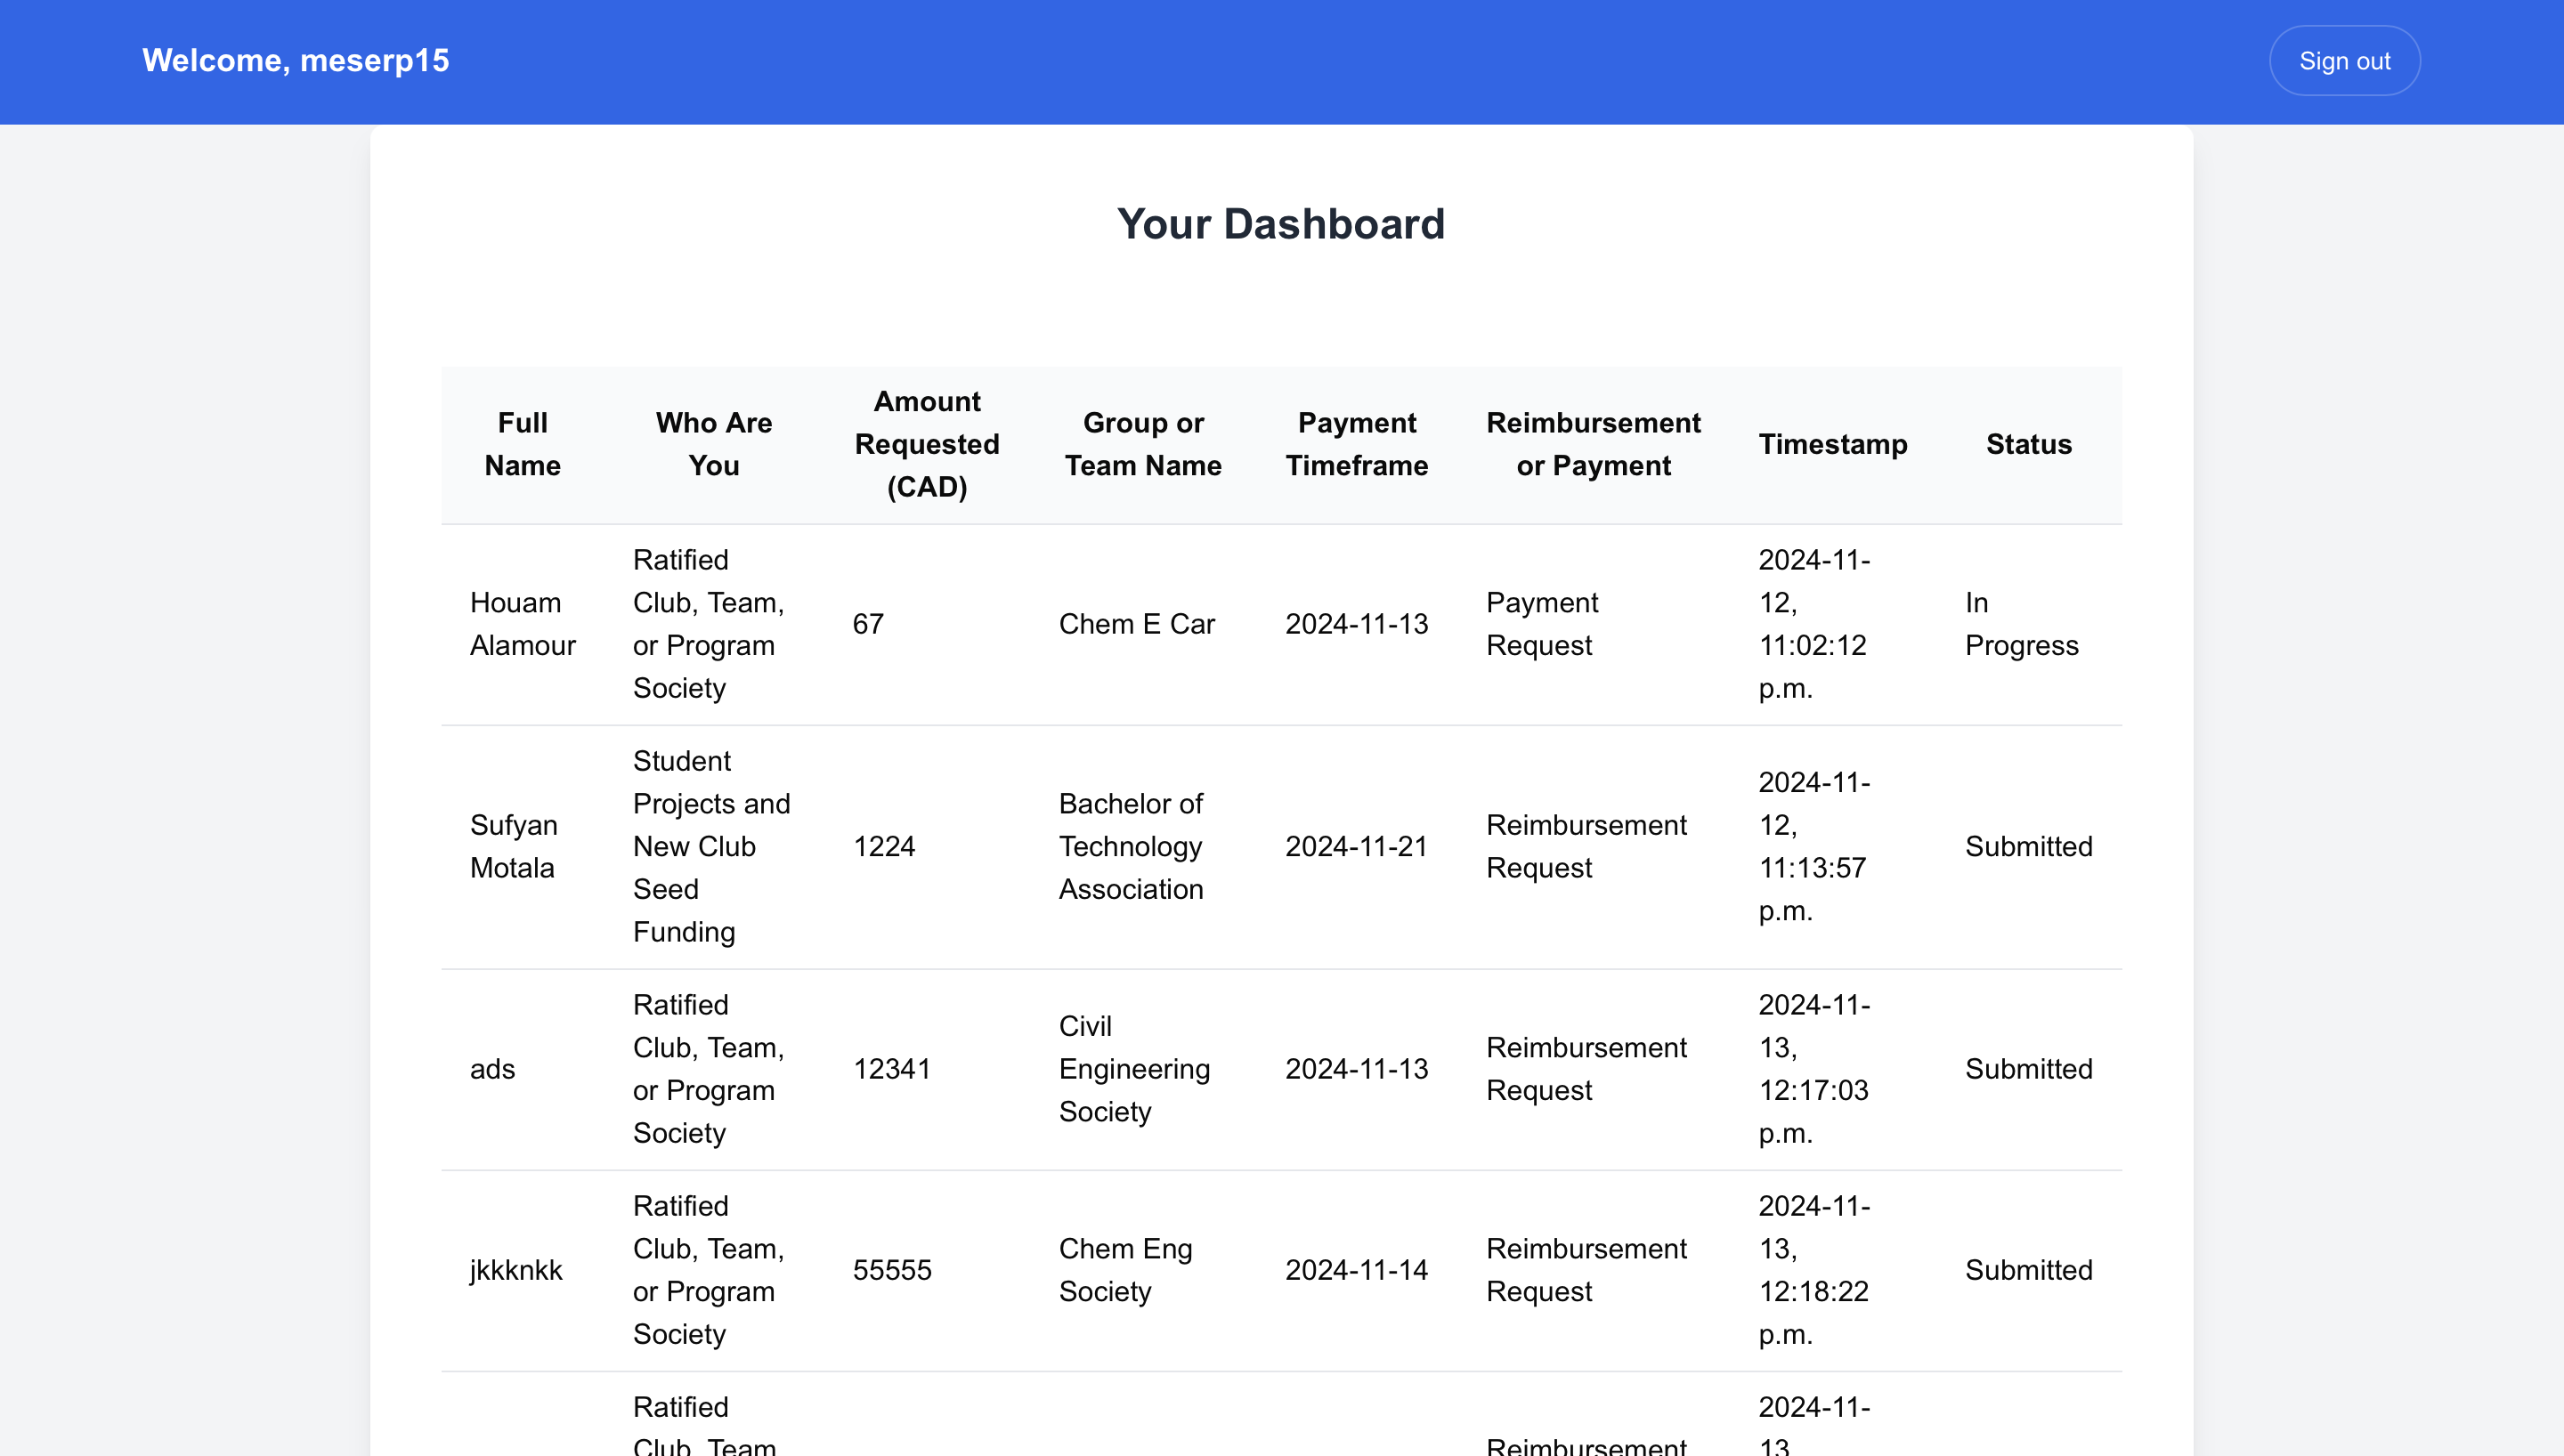
\includegraphics[width=0.8\textwidth]{img/dashboard.png}
    \caption{Dashboard View}
    \label{fig:dashboard}
\end{figure}

\subsection{Form}
\begin{figure}[H]
    \centering
    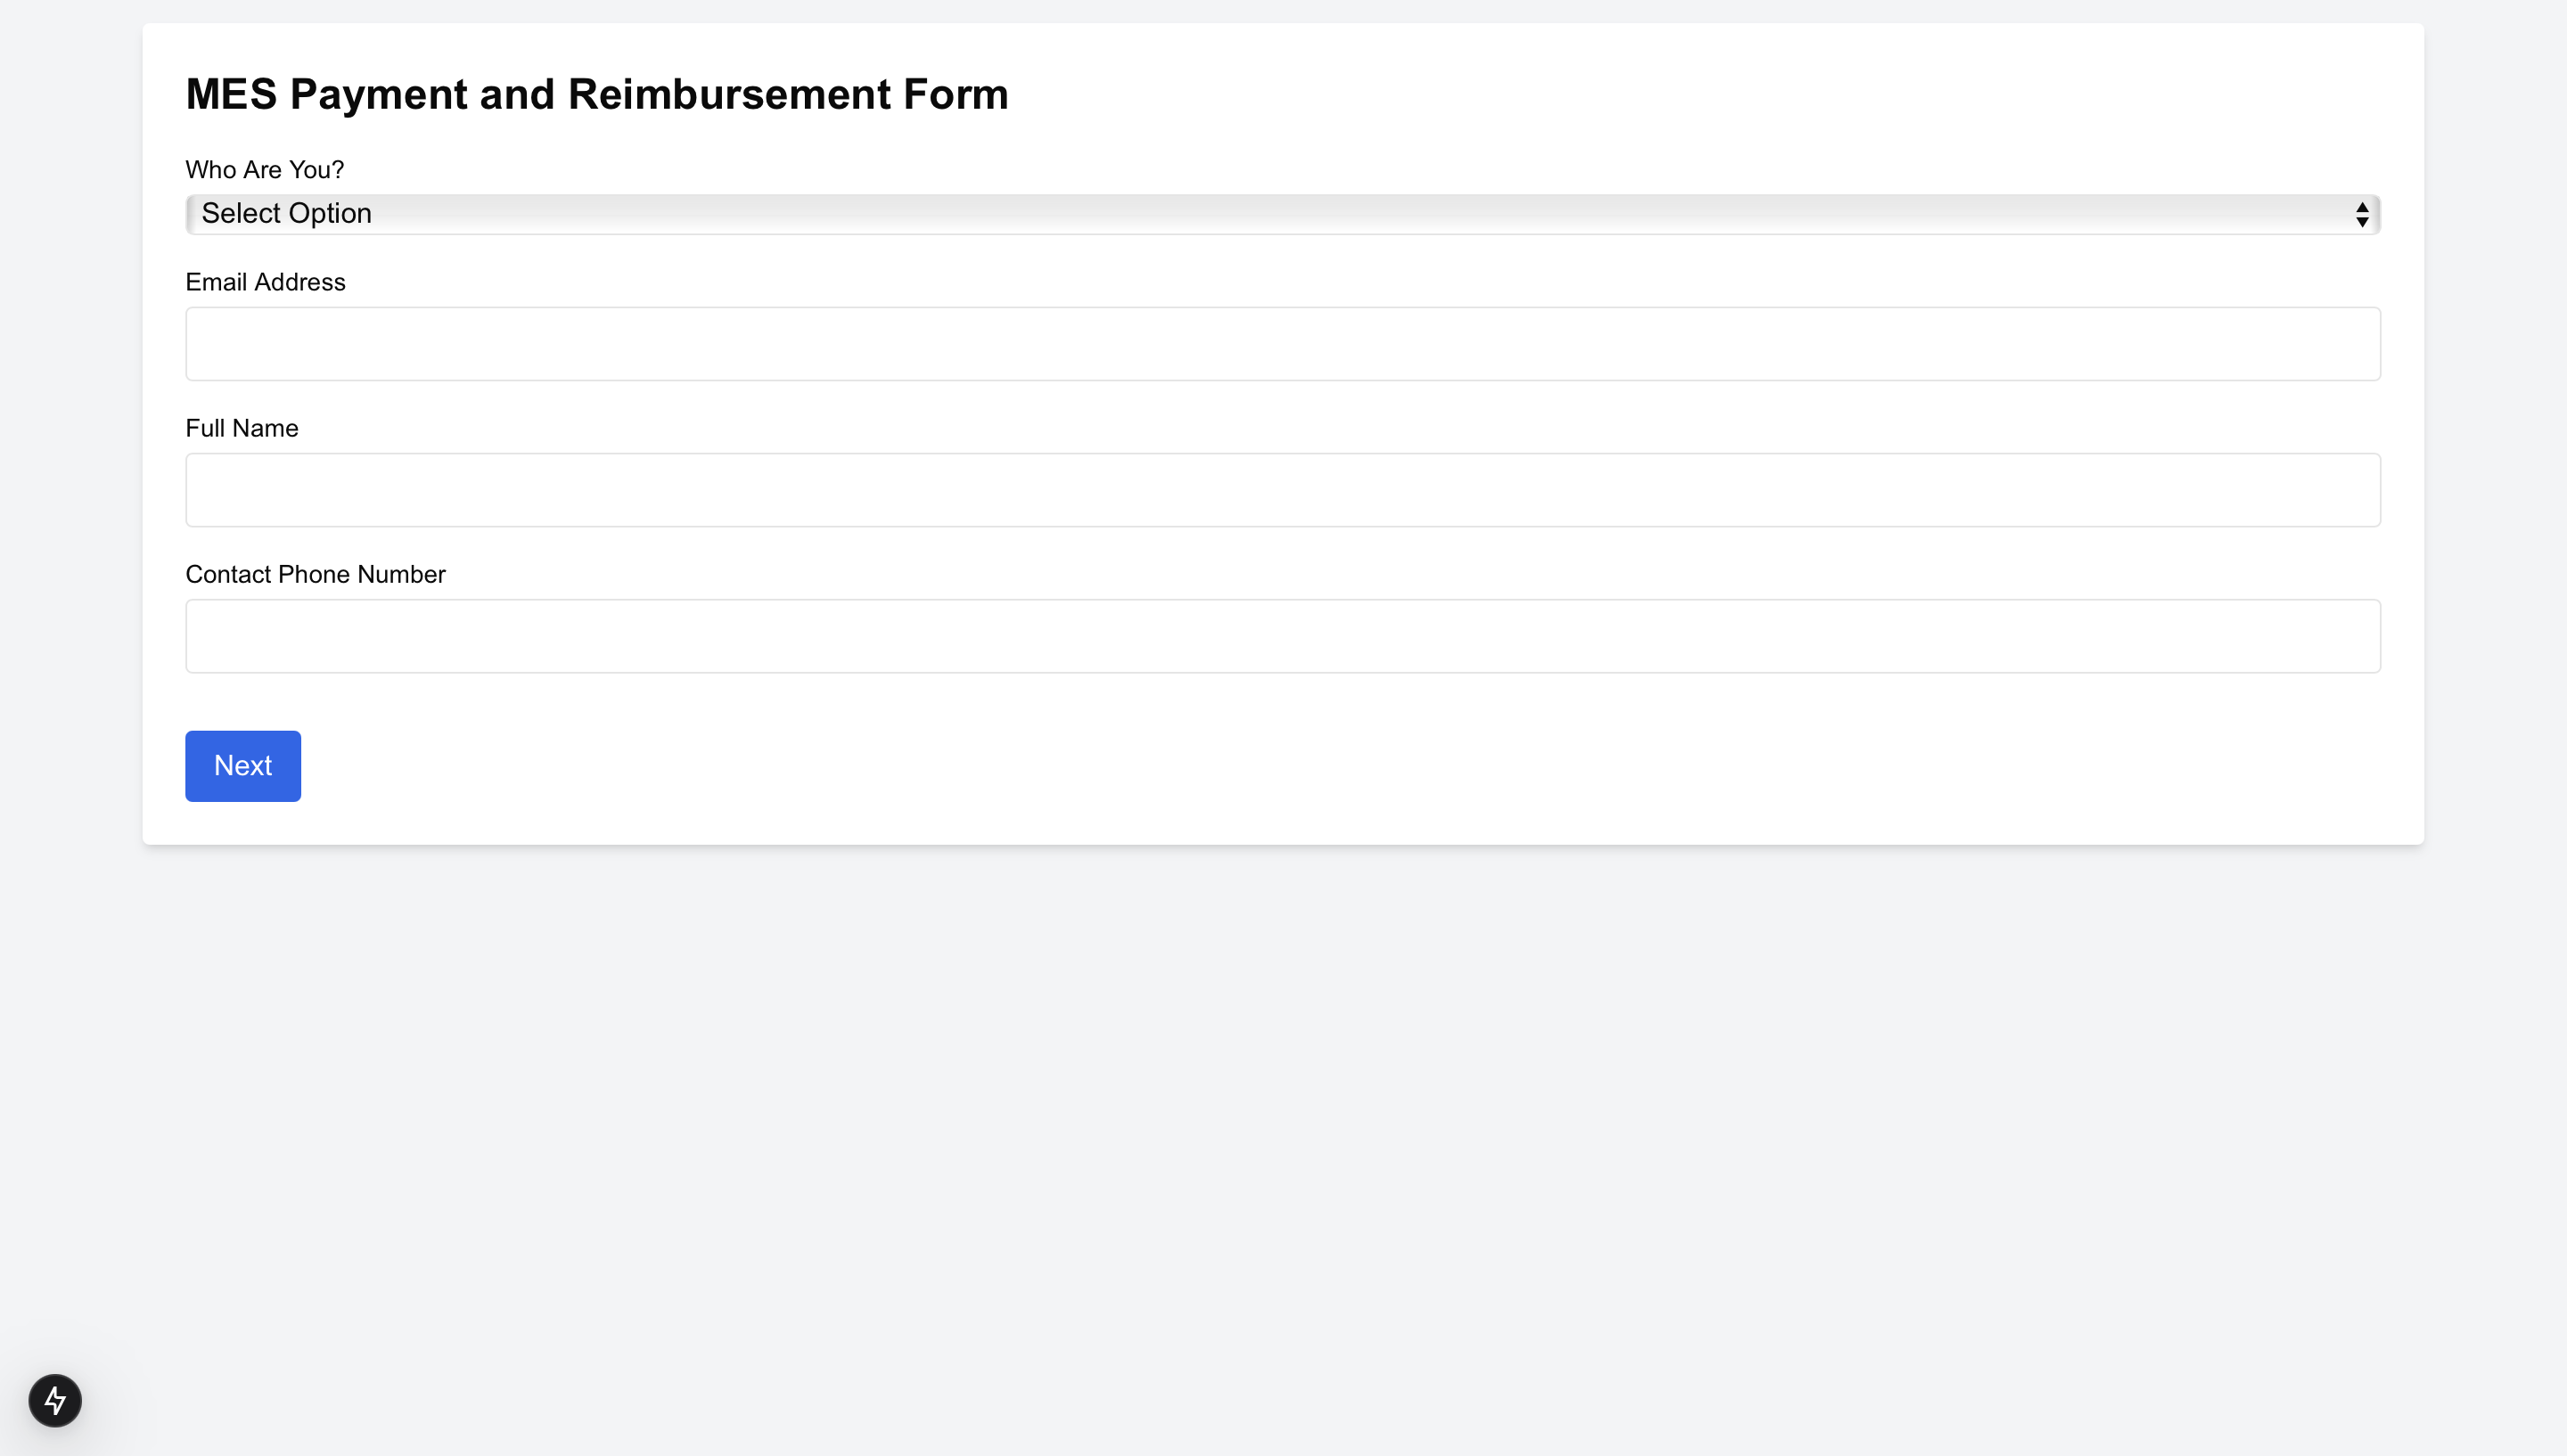
\includegraphics[width=0.8\textwidth]{img/form.png}
    \caption{Form View}
    \label{fig:form}
\end{figure}

\subsection{Login}
\begin{figure}[H]
    \centering
    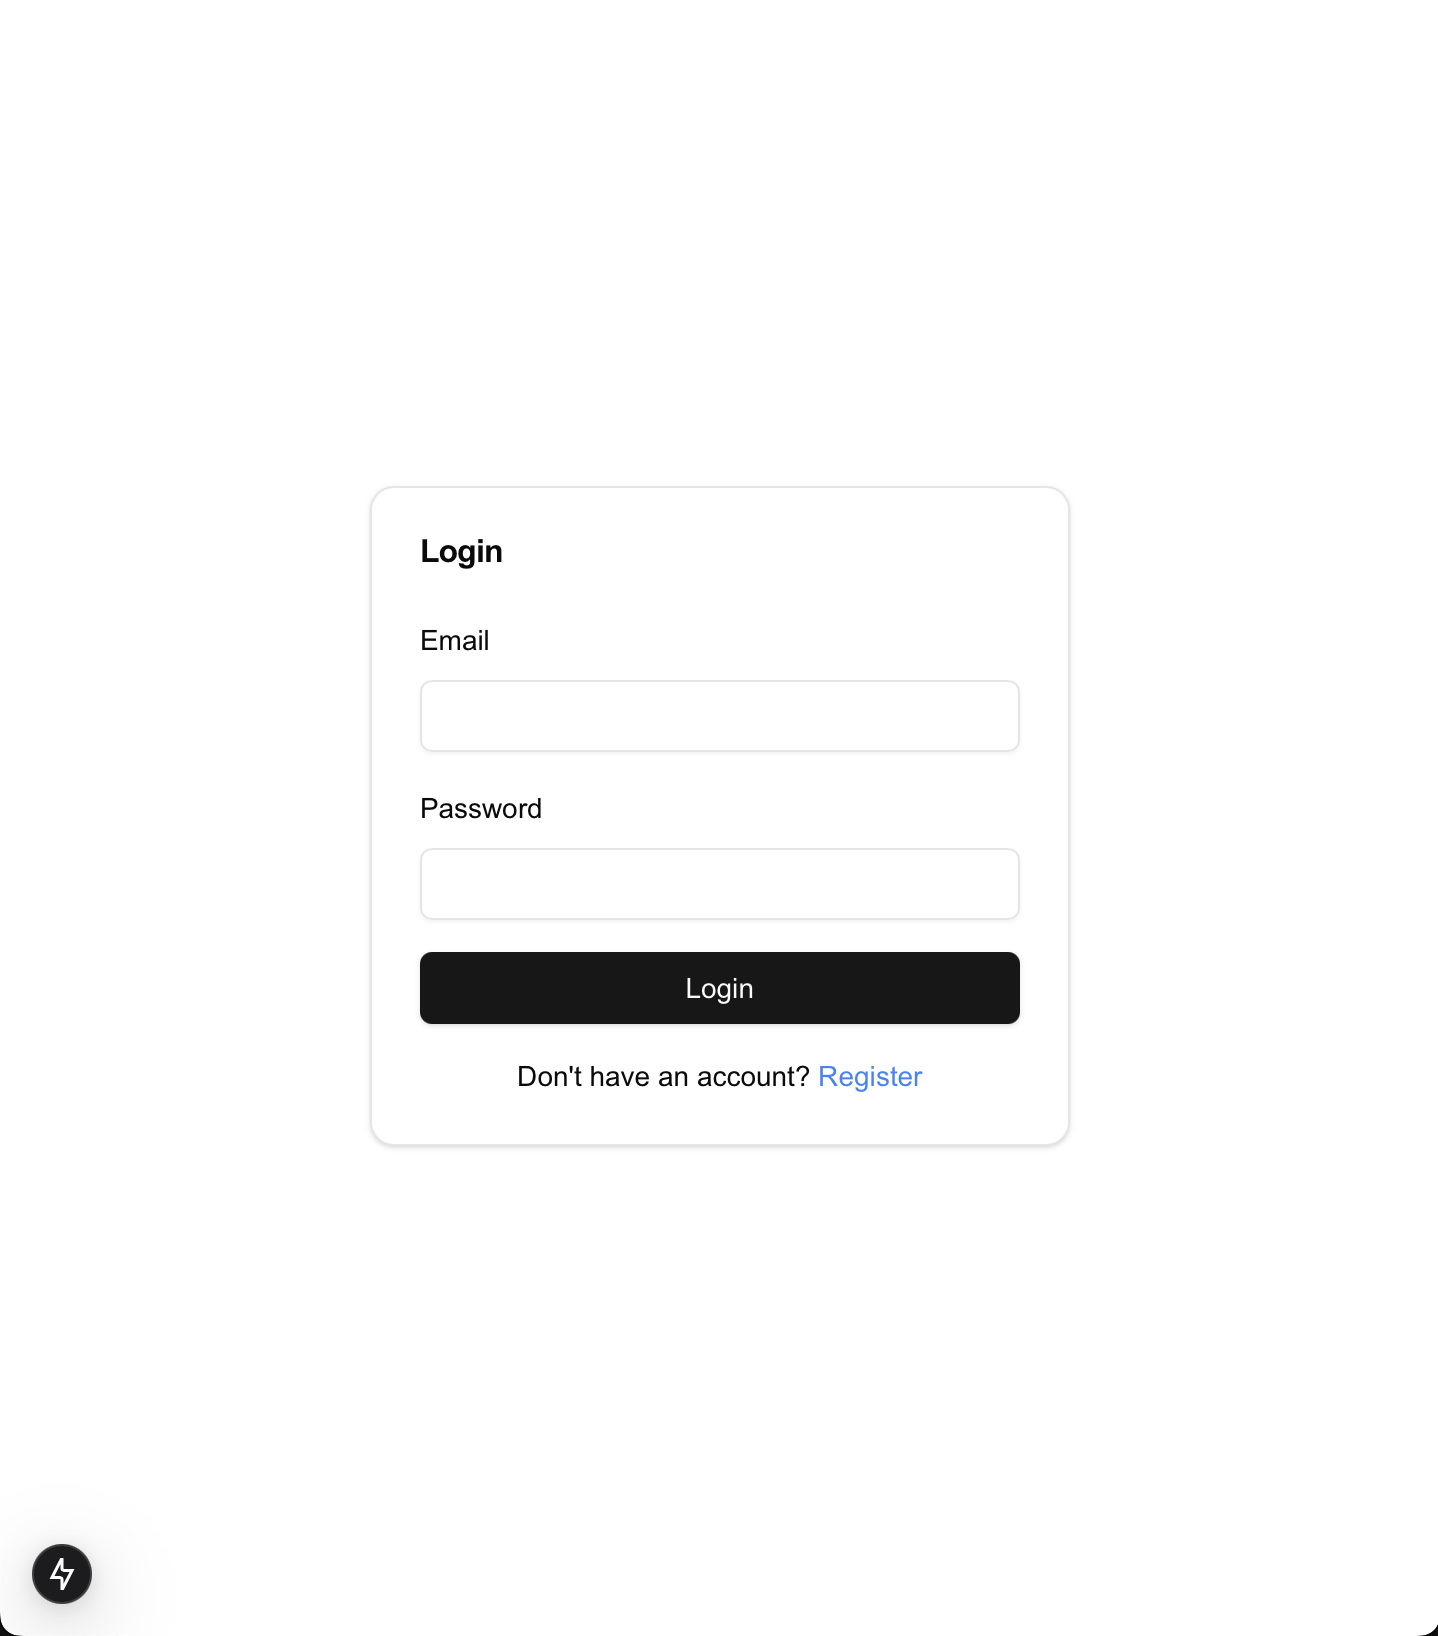
\includegraphics[width=0.8\textwidth]{img/login.png}
    \caption{Login View}
    \label{fig:login}
\end{figure}

\subsection{Receipt Input}
\begin{figure}[H]
    \centering
    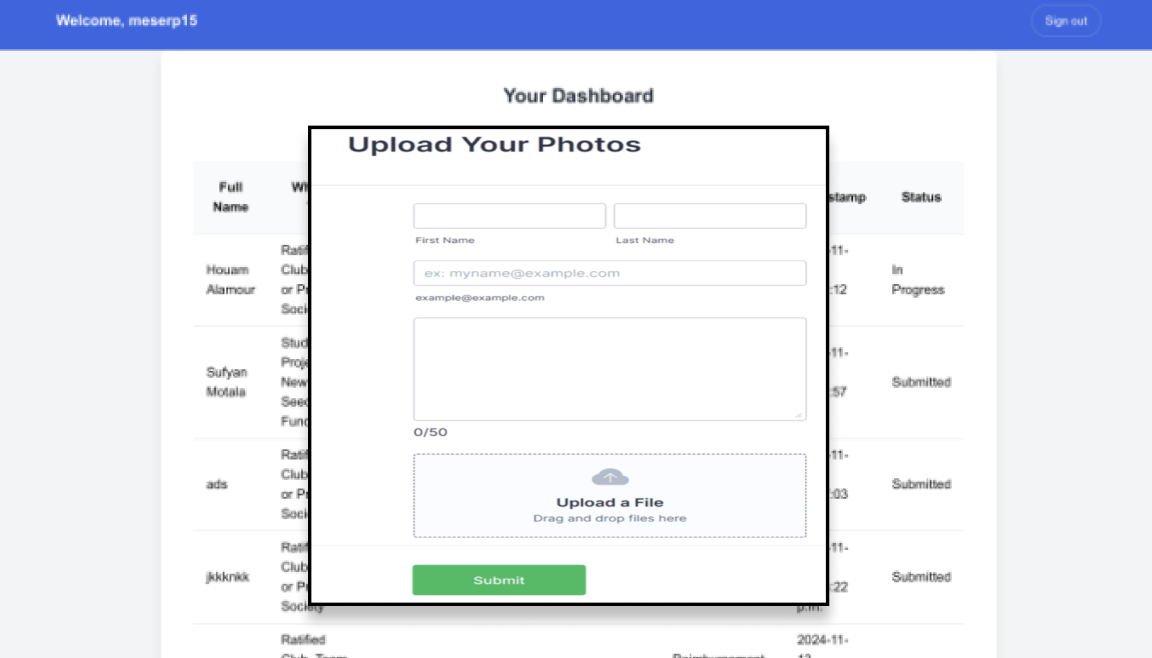
\includegraphics[width=0.8\textwidth]{img/upload.png}
    \caption{Receipt Scanning View}
    \label{fig:receipt}
\end{figure}

\subsection{Wesbsite Tutorial}
\begin{figure}[H]
    \centering
    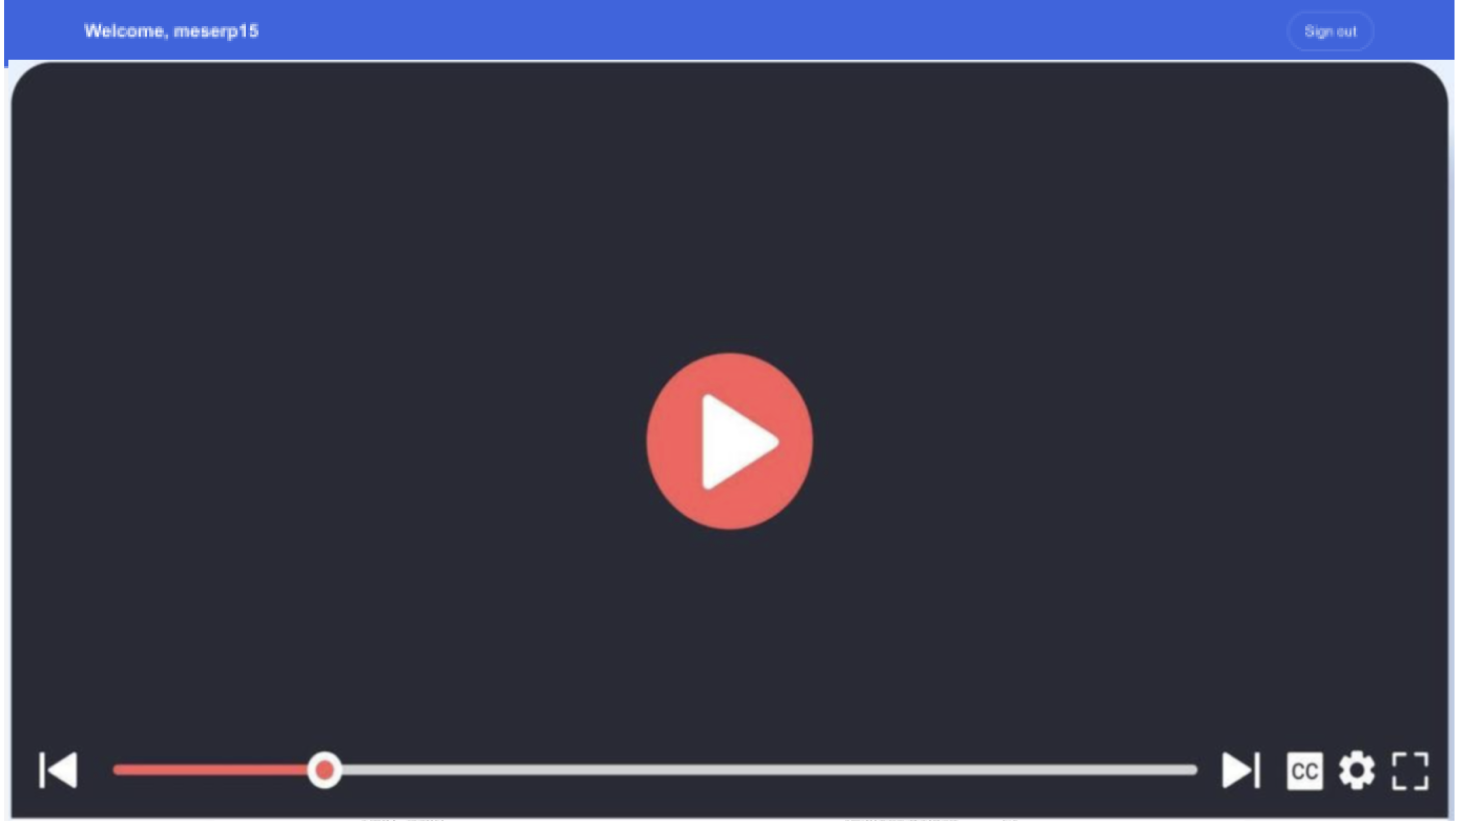
\includegraphics[width=0.8\textwidth]{img/tutorial.png}
    \caption{Tutorial Page}
    \label{fig:tutorial}
\end{figure}

\section{Design of Communication Protocols}

\begin{itemize}
  \item \textbf{APIs:} APIs will be used to communicate between the backend and the frontend of the application 
  \item \textbf{Email Registration:} When creating an account there will be email authentication to ensure valid users
  \item \textbf{Email communication:} When a reimbursement request is made or edited, the correct groups will be notified via email
\end{itemize}
\section{Timeline}

\begin{itemize}
  \item \textbf{Team Formed, Project Selected:} September 16 
  \begin{itemize}
    \item \textbf{All Team Members (Omar, Taaha, Rachid, Sufyan, Housam):} 
    Establish initial roles, select project scope, and identify stakeholder needs.
  \end{itemize}
  
  \item \textbf{Problem Statement, POC Plan, Development Plan:} September 23 
  \begin{itemize}
    \item \textbf{All Team Members:} 
    Finalize the problem statement for the MES-ERP system. Outline Proof-of-Concept (POC) objectives and develop a high-level development plan. 
    \item \textbf{Sufyan \& Omar:} Draft initial architecture sketches for key modules (Hardware-Hiding, Behaviour-Hiding, Software Decision).
  \end{itemize}
  
  \item \textbf{Requirements Document Revision 0:} October 9 
  \begin{itemize}
    \item \textbf{Housam \& Rachid:} Gather and refine user stories for Reimbursement Submission, Reimbursement Review, Budget Management, and Notification System.
    \item \textbf{Taaha:} Integrate feedback on Data Validation and Database Module requirements.
    \item \textbf{All Team Members:} Review and finalize the Requirements Specification for Rev 0.
  \end{itemize}
  
  \item \textbf{Hazard Analysis 0:} October 23 
  \begin{itemize}
    \item \textbf{Omar \& Sufyan:} Identify potential failure points for the Data Validation Module (e.g., corrupted or missing receipts) and the Database Module (e.g., concurrency issues).
    \item \textbf{Rachid:} Document mitigations for critical hazards in the Reimbursement Submission workflow (e.g., incorrect approvals).
  \end{itemize}
  
  \item \textbf{V\&V Plan Revision 0:} November 1 
  \begin{itemize}
    \item \textbf{Housam \& Taaha:} Draft initial testing approach for each module:
    \begin{itemize}
      \item \textbf{Hardware-Hiding Module:} Verify database connections and file I/O mocks.
      \item \textbf{Behaviour-Hiding Module:} Unit tests for Reimbursement Submission, Notifications, and Budget Dashboard.
      \item \textbf{Software Decision Module:} Automated tests for Data Validation, CI/CD, and Test Automation Framework.
    \end{itemize}
    \item \textbf{All Team Members:} Incorporate plan into the project schedule.
  \end{itemize}
  
  \item \textbf{Proof of Concept Demonstration:} November 11--22 
  \begin{itemize}
    \item \textbf{Omar, Taaha, Housam:} Implement a simplified Reimbursement Submission + Data Validation flow (happy path) for the demonstration.
    \item \textbf{Rachid \& Sufyan:} Set up the Database Module with mock data; create a minimal GUI prototype for user interaction.
    \item \textbf{All Team Members:} Conduct internal testing before the demonstration.
  \end{itemize}
  
  \item \textbf{Design Document Revision 0:} January 17
  \begin{itemize}
    \item \textbf{Omar \& Housam:} Document final architecture decisions for each module:
    \begin{itemize}
      \item \textbf{Hardware-Hiding Module:} Database and environment specifics.
      \item \textbf{Behaviour-Hiding Module:} Detailed class diagrams for Reimbursement, Notifications, and GUI.
      \item \textbf{Software Decision Module:} Data Validation logic and CI/CD pipeline configuration.
    \end{itemize}
    \item \textbf{Rachid \& Sufyan:} Cross-check design artifacts with SRS and POC feedback.
    \item \textbf{Taaha:} Integrate all design sections into a cohesive Revision 0 document.
  \end{itemize}
  
  \item \textbf{Revision 0 Demonstration:} February 3--February 14 
  \begin{itemize}
    \item \textbf{GUI Module (Rachid \& Sufyan):} Build an interactive front-end for Reimbursement Submission, including field-level validation feedback.
    \item \textbf{Data Validation Module (Taaha):} Finalize core validation checks (e.g., correct file formats, mandatory receipt uploads).
    \item \textbf{Reimbursement Review \& Approval (Omar):} Implement the basic approval workflow with role-based permissions.
    \item \textbf{Budget Dashboard (Housam):} Provide partial functionality (view-only) and real-time data fetch from the Database Module.
    \item \textbf{All Team Members:} Present Rev 0 to stakeholders, focusing on end-to-end demonstration of a reimbursement request.
  \end{itemize}
  
  \item \textbf{V\&V Report Revision 0:} March 7 
  \begin{itemize}
    \item \textbf{Taaha \& Omar:} Compile test results from module-level tests, including pass/fail statistics and coverage metrics.
    \item \textbf{Sufyan, Housam, Rachid:} Validate the correctness of reported bugs and retest major fixes in Reimbursement Submission and Budget Dashboard.
  \end{itemize}

  \item \textbf{Final Demonstration (Revision 1):} March 24--March 30 
  \begin{itemize}
    \item \textbf{All Team Members:} Incorporate feedback from Revision 0 and finalize all modules.
    \item \textbf{GUI Enhancements (Sufyan \& Rachid):} Polish front-end UX and incorporate advanced form validations for user-friendly error handling.
    \item \textbf{Notifications System (Housam):} Integrate push notifications and advanced triggers (e.g., overdue approvals).
  \end{itemize}
  
  \item \textbf{Add Receipt Scanning/Image Processing:} March 24--March 30 
  \begin{itemize}
    \item \textbf{Omar, Rachid, Housam:} Incorporate an OCR (Optical Character Recognition) service in the Reimbursement Submission module. 
    \item \textbf{Taaha:} Update the Data Validation Module to handle scanned data edge cases (e.g., partial text scans).
  \end{itemize}
  
  \item \textbf{Add User Manual to Application:} March 24--March 30 
  \begin{itemize}
    \item \textbf{Sufyan:} Create comprehensive end-user documentation and how-to guides, focusing on reimbursements and approvals.
    \item \textbf{All Team Members:} Review for clarity and completeness before final release.
  \end{itemize}
  
  \item \textbf{Refine the UI, Functions, and Backend Connectivity:} March 24--March 30 
  \begin{itemize}
    \item \textbf{Taaha:} Implement advanced error handling across all modules and polish backend endpoints for reliability.
    \item \textbf{All Team Members:} Conduct integration testing for the updated features.
  \end{itemize}
  
  \item \textbf{Reach Out to MES Rep (Weekly):} March 24--March 30 
  \begin{itemize}
    \item \textbf{Omar, Taaha, Rachid, Sufyan, Housam:} Schedule status meetings, collect user feedback, and prioritize final tweaks for Rev 1.
  \end{itemize}
  
  \item \textbf{EXPO Demonstration:} April (TBD) 
  \begin{itemize}
    \item \textbf{All Team Members:} Showcase the fully functional application, highlighting compliance auditing, budgeting, and user flows.
  \end{itemize}

  \item \textbf{Final Documentation (Revision 1):} April 2 
  \begin{itemize}
    \item \textbf{All Team Members:} Update the Design Document, MG, MIS, V\&V Report, and User Manual with final revisions and new features.
    \item \textbf{Omar \& Taaha:} Proofread overall consistency and finalize submission to the department.
  \end{itemize}
\end{itemize}


\bibliographystyle {plainnat}
\bibliography{../../../refs/References}

\newpage{}

\end{document}